%!TEX root = ../main.tex
% !TeX spellcheck = en_GB 
% Chapter 2
%------------------------------------------------------------------------------------
\chapter{Unmanned Surface Vehicles} % Main chapter title

\label{Unmanned_Surface_Vehicles} % For referencing the chapter elsewhere, use \ref{Chapter1}
%------------------------------------------------------------------------------------


Unmanned Surface Vehicles (USV) or Autonomous Surface Crafts (ASC) are vehicles operating the seas without a crew on-board.
USVs encompass both fully autonomous vehicles, from now on referred to as ASCs, and semi-autonomous vehicles.
Development of USVs has been ongoing for the last two decades \cite{manley2008unmanned}.
However, the majority of the USVs developed are of the semi-autonomous type \cite{liu2016unmanned,park2017development}, meaning that they depend on human intervention to some extent usually by a supervisor located on shore.
Although semi-autonomous USVs greatly increase the safety of the operating personnel \cite{liu2016unmanned}, they do not completely remove the need for human interaction.
Supervision of several semi-autonomous vehicles can be admittedly be handled by a single person, which significantly decreases the number of person-hours needed to accomplish a specific mission \cite{manley2008unmanned}.
The person-hours needed for surveillance could, however, be removed completely by a ASC.
It is, therefore, of great interest to overcome the challenges associated with ASCs.


%------------------------------------------------------------------------------------
\section{Usage}
\textcite{Yuh2011} mention that roughly two-thirds of the earth's surface is covered by water, with an average depth of the oceans being 3688 m \cite{depth_ocean}.
Thereby, adding up to a vast amount of explorable areas of which 95 \% is yet to be seen by human eyes \cite{explored_percentage}. Utilization of autonomous vehicles could notably facilitate the  exploration of these, yet unknown, areas.
Although ASCs are situated on the surface of the ocean they can greatly increase the efficiency of Unmanned Underwater Vehicles (UUV) by acting as a gateway between UUVs and services, such as GPS, not easily available in underwater environments \cite{liu2016unmanned}.

\textcite{liu2016unmanned} have, furthermore, compiled a list of potential applications of USVs, along with previous research on the topics.
The list is divided into five major categories: scientific research, environmental missions, ocean resource exploration, military use, and other applications.

\section{Advantages}
\todo{More advantages}
USVs have, apart from the obvious decrease in man hours, a few advantages over traditional manned vessels. The absence of humans on board means that facilities and resources such as canteens,  manned bridges, showers etc. are no longer needed. The weight saved increases the manoeuvrability and deployability and can also be used to increase the payload the vessel is able to carry. USVs can, furthermore, conduct longer and more hazardous voyages than manned vessels since the personnel is located safely on land. This has the additional benefit of decreasing the operational costs \cite{liu2016unmanned}.

%\subsection{Current state}
%------------------------------------------------------------------------------------
\section{Challenges}
Even though USVs bring many advantages to the maritime industry, there are still quite a few challenges that need to be solved. The following section presents some of these challenges and their relation to the scope of this thesis.


USVs should be able to operate in a highly variable environment, all over the world, in terms of climate, traffic density and communication channels available.  Algorithms and systems developed should, therefore, ideally be usable in all situations that might arise in this environment. This introduces challenges both hardware and software wise \cite{liu2016unmanned}. The limited scope of this thesis narrows the research to only the software related challenges with a focus on path planning, especially collision avoidance.

All vessels operating on water are bound to follow the international maritime "Rules of the Road" called the Convention on the International Regulations for Preventing Collisions at Sea, 1972 (COLREGs) explained in section \ref{sec_colreg}. This is also true for USVs, since they should be able to operate in situations that comprise both other USVs and manned vessels that follow the COLREGs rules. Furthermore, they should be able to  act in a safe manner in situations where other vessels, for some reason, are not complying with the COLREGs rules. Hence, it is crucial for the USVs to follow COLREGs to ensure safe operations.

COLREGs were originally introduced in 1972, to reduce the amount of collisions at sea. They are written to be interpreted by humans. Situations where multiple rules apply and contradict each other might therefore arise. These situations are usually solved with the use of good seamanship and human deduction. These aspects pose challenges when translating the COLREGs rules into computer understandable code \cite{benjamin2006method}.


%------------------------------------------------------------------------------------
\chapter{COLREG}
\label{sec_colreg}
The Convention on the International Regulations for Preventing Collisions at Sea, 1972 (COLREGs) were adopted 1972 and entered into force 1977 in it's original form. COLREGs consist of 38 rules, grouped into five different sections as is designed by the International Maritime Organization (IMO).
The original objective of COLREGs was to ensure traffic separation between maritime vessels in an increasingly populated environment back in 1972 and it is, therefore, sometimes referred to as the Rules of the Road for maritime vessels. COLREGs have since then been in use and is still mandatory to adhere to on international waters. However, a great deal has changed since the COLREGs initially entered into force and COLREGs has, therefore,
received amendments several times \cite{colreg_about_imo}.

National regulations might differ from the COLREGs to some extent. However, COLREGs mention that ‘Nothing in these Rules shall interfere with the operation of special rules made by an appropriate authority for roadsteads, harbours, rivers, lakes or inland waterways connected with the high seas and navigable by seagoing vessels.
Such special rules shall conform as closely as possible to these Rules.’ \cite{colreg}

%------------------------------------------------------------------------------------
The following sections will present the different parts of the COLREGs regulations, with emphasis on the parts related to manoeuvring a USV in international waters. Information in this subsection is taken from the official COLREGs regulations  \cite{colreg} if not otherwise specified. Part D and E will not be discussed further, since they are not of interest for the scope of this thesis. Moreover, rules that are not of interest for the scope of this thesis will not be mentioned.
%------------------------------------------------------------------------------------
\section{Part A General}

Part A consist of three rules and address general conditions when and to which vessels COLREGs apply. This includes all vessels navigating on high seas and all waters connected therewith. Additionally, it specifies that special rules regarding roadsteads, harbours, rivers, lakes or inland waterways connected with the high seas and navigable by seagoing vessels shall conform as closely as possible to these Rules (\textit{Rule1}). Furthermore words, such as vessel, power-driven vessel, sailing vessel, length, breadth, and other words used in the regulations are defined (\textit{Rule3}). Finally, it is stated that the COLREGs rules do not in any way free the vessel, owner, master or crew from responsibility to follow the rules and act according to the ordinary practice of seamen (\textit{Rule2}).

%------------------------------------------------------------------------------------
\section{Part B Steering and Sailing}
Part B is split up into three different sections. The first section consists of rules \todo{words or numerals} 4-10 and apply in any condition of visibility. Section II (rules 11-18) apply to vessels in sight of each other, while the last section consist of just one rule that specifies reduced visibility operations. It states that vessels should proceed at speeds appropriate to the circumstances and use radar to determine collision risks. Speed should be reduced to a minimum if a vessel can hear another vessels fog horn apparently forward of her beam (\textit{Rule19}).

Section I addresses how vessels shall operate in order to ensure proper situational awareness with emphasis on collision risk detection.  It is mandatory for  all vessels to at all times maintain proper look-out by sight and hearing and all other available means to ensure the best possible situational awareness (\textit{Rule5}) and use all means possible to determine if a risk of collision exists. This includes the use of radar equipment although caution should be exercised not to trust insufficient data. A collision is considered to be imminent when two vessel maintain constant compass bearings to each other over a prolonged time.
However, a constant bearing is only a sufficient condition for a collision risk, not a necessary one. Close range, large vessels or a tow might pose a collision risk without a constant bearing. Moreover, it is stated that any doubt whether a risk of collision exists shall be treated as if a risk exists (\textit{Rule7}).
Vessels shall, furthermore, maintain a speed so that they can take proper and effective action to avoid a collision and stop within a distance appropriate to the prevailing circumstances and conditions (\textit{Rule 6}). Any actions made in order to to avoid collisions shall, additionally, be taken according to the rules and as far as possible be conducted in ample time and large enough so that they are easily observable by other vessels. Small alterations should, in other words, be avoided. Course alterations might also be accompanied by a lowering of speed, if considered necessary to ensure that the vessels pass each other at safe distance (\textit{Rule 8}).

Section II defines three different scenarios, involving two vessels, and specifies the action to take for both vessel. The scenarios are a head-on, a crossing and an overtake situation. A vessel overtaking another vessel shall keep out of the way of the stand on vessel. A vessel is considered to overtake another vessel when approaching it from a direction more than 22.5 \textdegree abaft the stand on vessels beam, i.e with a relative bearing between 112,5 \textdegree and 247,5 \textdegree from the stand on vessel (\textit{Rule 13}). A head-on situation, on the other hand, is when a vessel sees another vessel ahead or nearly ahead, i.e. it can see the masthead light in line or both sidelights. The give way vessel shall, in this case, alter its course to starboard (\textit{Rule 14}). Finally it is stated that vessel coming from starboard, i.e right, has the right of way in a crossing situation. The give way vessel shall if possible avoid crossing ahead of the other vessel and, therefore, alter its course to starboard  (\textit{Rule 15}). All actions by the give away vessels shall be taken as early as possible  (\textit{Rule 16}), while the stand on vessels shall keep its course and speed, provided that the give way vessel acts according to the regulations. However, the stand on vessel might take action to best avoid a collision if it finds that the actions by the give way vessels are insufficient to prevent a collision  (\textit{Rule 17}). Responsibilities between vessels of different types are also addressed. For instance, a power-driven vessel shall give way for a vessel engaged in fishing  (\textit{Rule 18}).

%------------------------------------------------------------------------------------
\section{Part C Lights and Shapes}
\begin{figure}[H]
    \centering
    \includegraphics[width=0.5\textwidth]{Figures/lights}
    \caption{Mandatory navigation lights}
    \label{fig:nav_lights}
\end{figure}

Part C specifies the lights and shapes a vessel shall exhibit, and when they should be used. These are therefore not of interest for the scope of this thesis, with the exception of \textit{rule 21} and \textit{rule 22}, which specify the arcs that specific lights should cover as well as the distance the should be visible from. Figure \ref{fig:nav_lights} shows the lights of interest for this thesis.
\\
\textbf{Masthead lights} cover a 225 \textdegree arc from 247,5 \textdegree to 112,5 \textdegree and should be visible from at least 2-6 miles, depending on the length of the vessel.\\
\textbf{Sidelights} are green on the starboard side and red on port. They cover a 112,5 arc from 0 relative bearing to 112,5 and 247,5 respectively. They should be visible from at least 1-3 miles, depending on the length of the vessel.

-------------------------------------------------------------------------

\chapter{Alternative COLREG compliant algorithms}
USVs have been in development since at least 1993 when MIT started its Sea Grant College Program, Autonomous Surface Craft (ASCs) \cite{manley2008unmanned}. Many different approaches and algorithms have since then been tried out. This section will briefly look into some of the COLREGs compliant approaches, before finally presenting the approach which this thesis is based on.


\textcite{larson2007advances} uses a two-level two-dimensional obstacle map to create a near-field reactive control technique. One layer for a near field model and the other for a far field model. COLREGs rules are incorporated into the solution by utilizing a rule-based approach in the path planner. The solution is made with computational efficiency in mind and the provided trajectory is, therefore, not optimal. It is also stated that the sensors and processing algorithm need more work. However, the authors have plane for future improvements and the algorithm is regularly tested in San Diego Bay.


Another approach, developed by \textcite{benjamin2004colregs,benjamin2006method} utilizes multi-objective optimization and interval programming, within a behaviour based architecture. The solution has been tested with kayak-based autonomous surface crafts and initial tests show promising results, but the solution cannot yet be called COLREGS compliant.


\textcite{naeem2012colregs}
propose a path-planer that uses line of sight guidance between way-points. Obstacles are avoided by introducing a starboard heading bias to the line of sight heading until clear of conflict. The paper compares the trajectory, produced by the proposed on-the-fly algorithm, to that of a modified off-line DPSS strategy. Multiple simulations show that both algorithms yield COLREGs compliant results. However, a simulation with multiple dynamic targets was not conducted.

Spatio temporal reasoning have also been considered as an way to translate the COLREG rules into computer understandable rules. \textcite{spat_temp1,spat_temp2}
suggest the use of Oriented Point Reasoning Algebra (OPRA) with \textit{m}  granularity to represent vessels position and relative moving direction.
A qualitative spatio-temporal reasoning toolbox is used to convert the geometric scenario consisting of the vessels Cartesian coordinates into a qualitative scene description based of OPRA relations. The same toolbox can then generate all possible scenarios that are spatially or temporally possible. Model checking can then be conducted on the  observations to check whether the behaviour of the involved vessels is  COREGS compliant.


\textcite{lee2004fuzzy} combine fuzzy logic with modified virtual force fields to  create a COLREGs compliant algorithm. The fuzzy logic rule-set used consists of about two hundred rules, which might be computational challenging. The authors do, however, mention that the rules-set might be streamlined. Fuzzy logic is also used \textcite{perera2012intelligent} which, furthermore uses bayesian networks to solve cases with multiple target vessels. The presented simulations consist of one vessel utilizing the algorithm to avoid three dummy vessels that are keeping their course and speed. The rule-set is in this paper also quite extensive.


Both fuzzy logic and spatio temporal reasoning with model checking was considered to be used as the foundation for this thesis. However, fuzzy logic was finally chosen due to the fact that the qualitative representation of a scenario in spatio temporal reasoning is limited the definitions of the calculus used, in this case OPRA.
%------------------------------------------------------------------------------------
\chapter{Fuzzy set theory and logic}
The concept of fuzzy sets was first mentioned by \textcite{zadeh1996fuzzy} in 1964 as a way of dealing with sets of objects, where an objects membership to a set can be represented by a value in the real interval [0, 1]. Compared to classic set theory where  membership is restricted to the two values of one and zero. Fuzzy logic enables one to define sets such as "old men" or "vessels on reciprocal course" \cite{zadeh1996fuzzy}, which facilitates the process of converting human abstract reasoning into computer understandable logic.
%------------------------------------------------------------------------------------
\section{Fuzzy sets}
The fuzzy set "all old men" can be defined in the following way. Let the \textit{universe set} \textbf{X} be the set of ages [0, 100]. The set of old men can then be written as
$\fuzzyset{A}=\left \{ a \in \textbf{X} | a \text{ is old} \right \}$
\cite{chen2000introduction}

However, the set requirement 'is old' is still undefined and therefore vague. Defining the threshold of being old at an age of 60 does divide the universal set \textbf{X} into subsets of 'old' and 'not old', but the division does not distinguish between humans aged 1 and 59.
Fuzzy set theory introduces the concept of membership functions, to solve this problem. A Fuzzy Membership Function (FMF) describes the grade of membership of a  in  $\fuzzyset{A}$. This function is often written as $\mu_{\fuzzyset{A}}(a)$. Figure \ref{fig:FMF_ex} shows a very simple linear FMF for the example $\fuzzyset{A}=\left \{\text{'is old'} \right \}$, where for instance $\mu_{\fuzzyset{A}}(10)=0.1$. Similar FMFs can be defined for young and middle-aged which results in the graph seen in figure \ref{fig:FMF_ex2} \cite{ross2009fuzzy}.

A fuzzy set can then be written as an array of tuples consisting of the objects and its associated membership value: $\fuzzyset{A}=\left \{(x,\mu_{\fuzzyset{A}}(x)|x \in X) \right \}$ \cite{zimmermann2010fuzzy}, which gives \\ $\fuzzyset{A}=\left \{(0,1),(10,0.9),(20,0.8),\dots,(90,0.1),(100,0) \right \}$ for the example $\fuzzyset{A}$=\{'is young'\} in figure \ref{fig:FMF_ex} \cite{ross2009fuzzy}.

\begin{figure}[H]
    \centering
    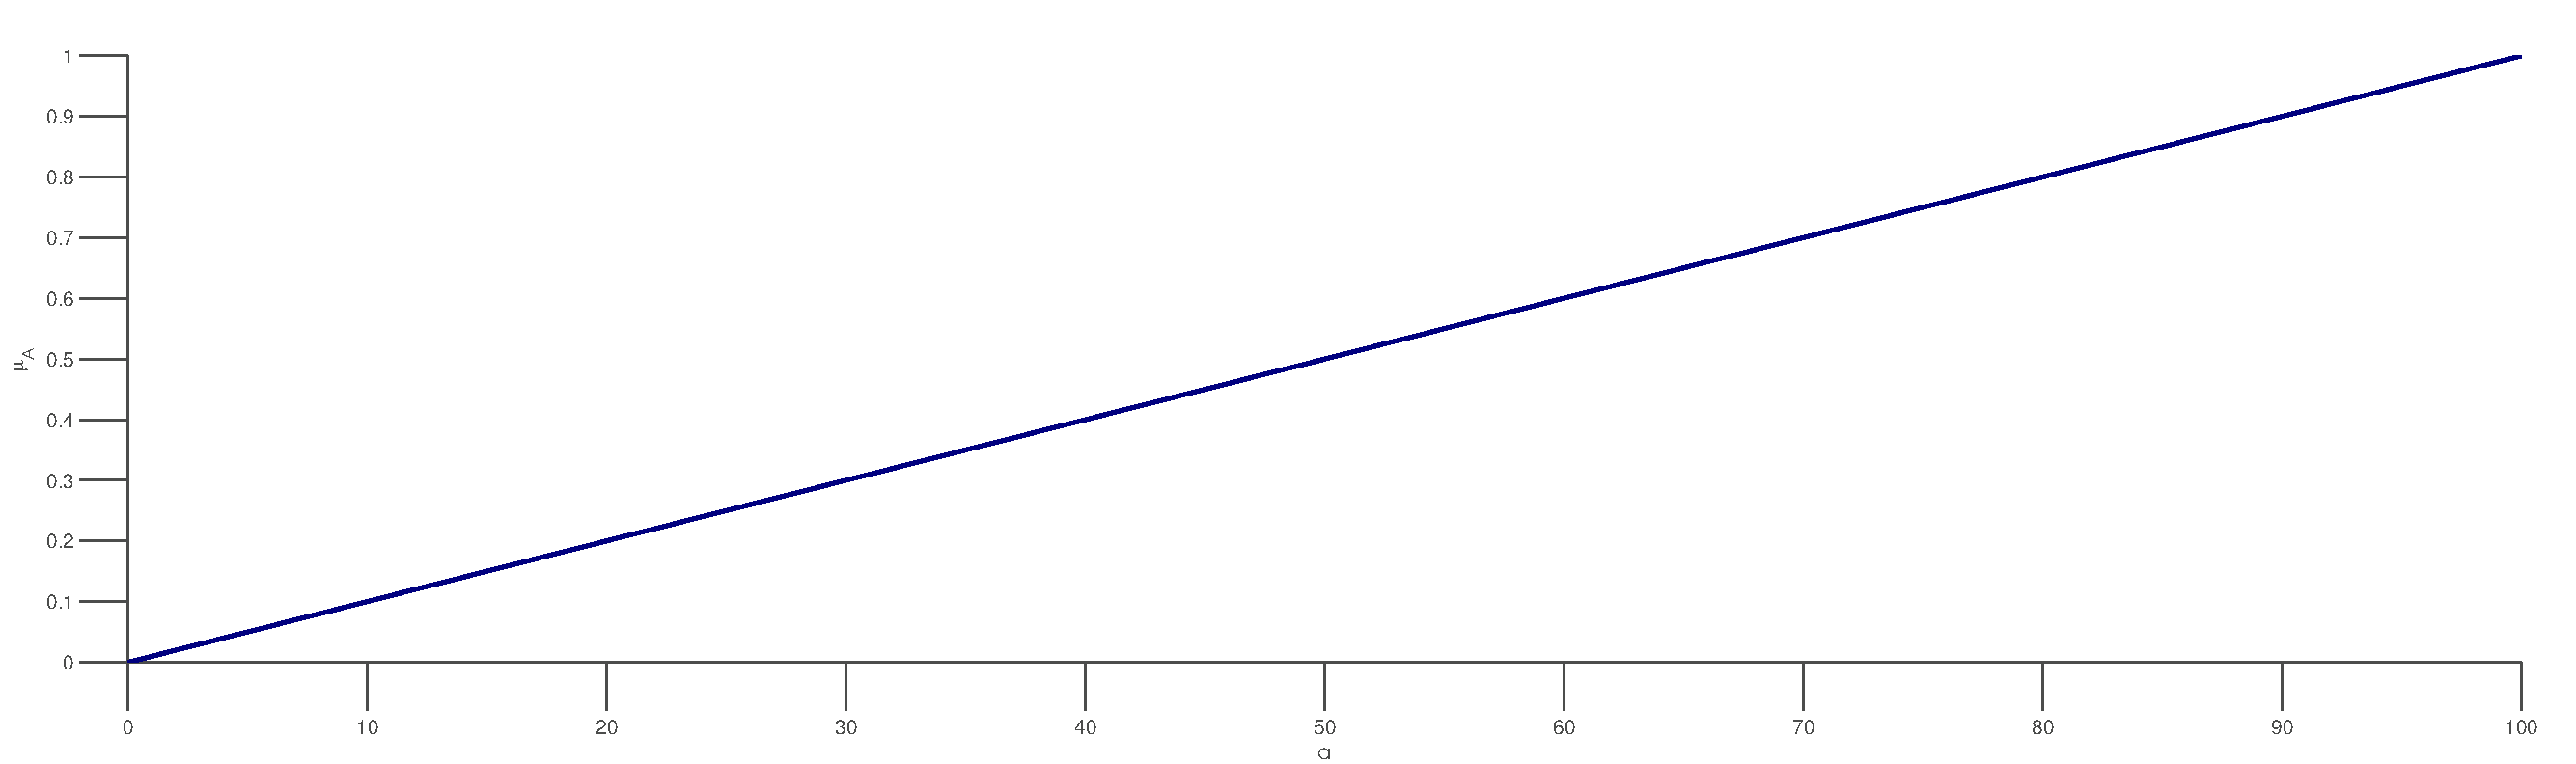
\includegraphics[width=\textwidth]{FMF_ex}
    \caption[Graphical representation of a single FMF]{Fuzzy membership function for $\protect\fuzzyset{A}=\left \{ \text{'Is old'} \right \}$}
    \label{fig:FMF_ex}
\end{figure}
\todo{Increase graphic font}
\begin{figure}[H]
    \centering
    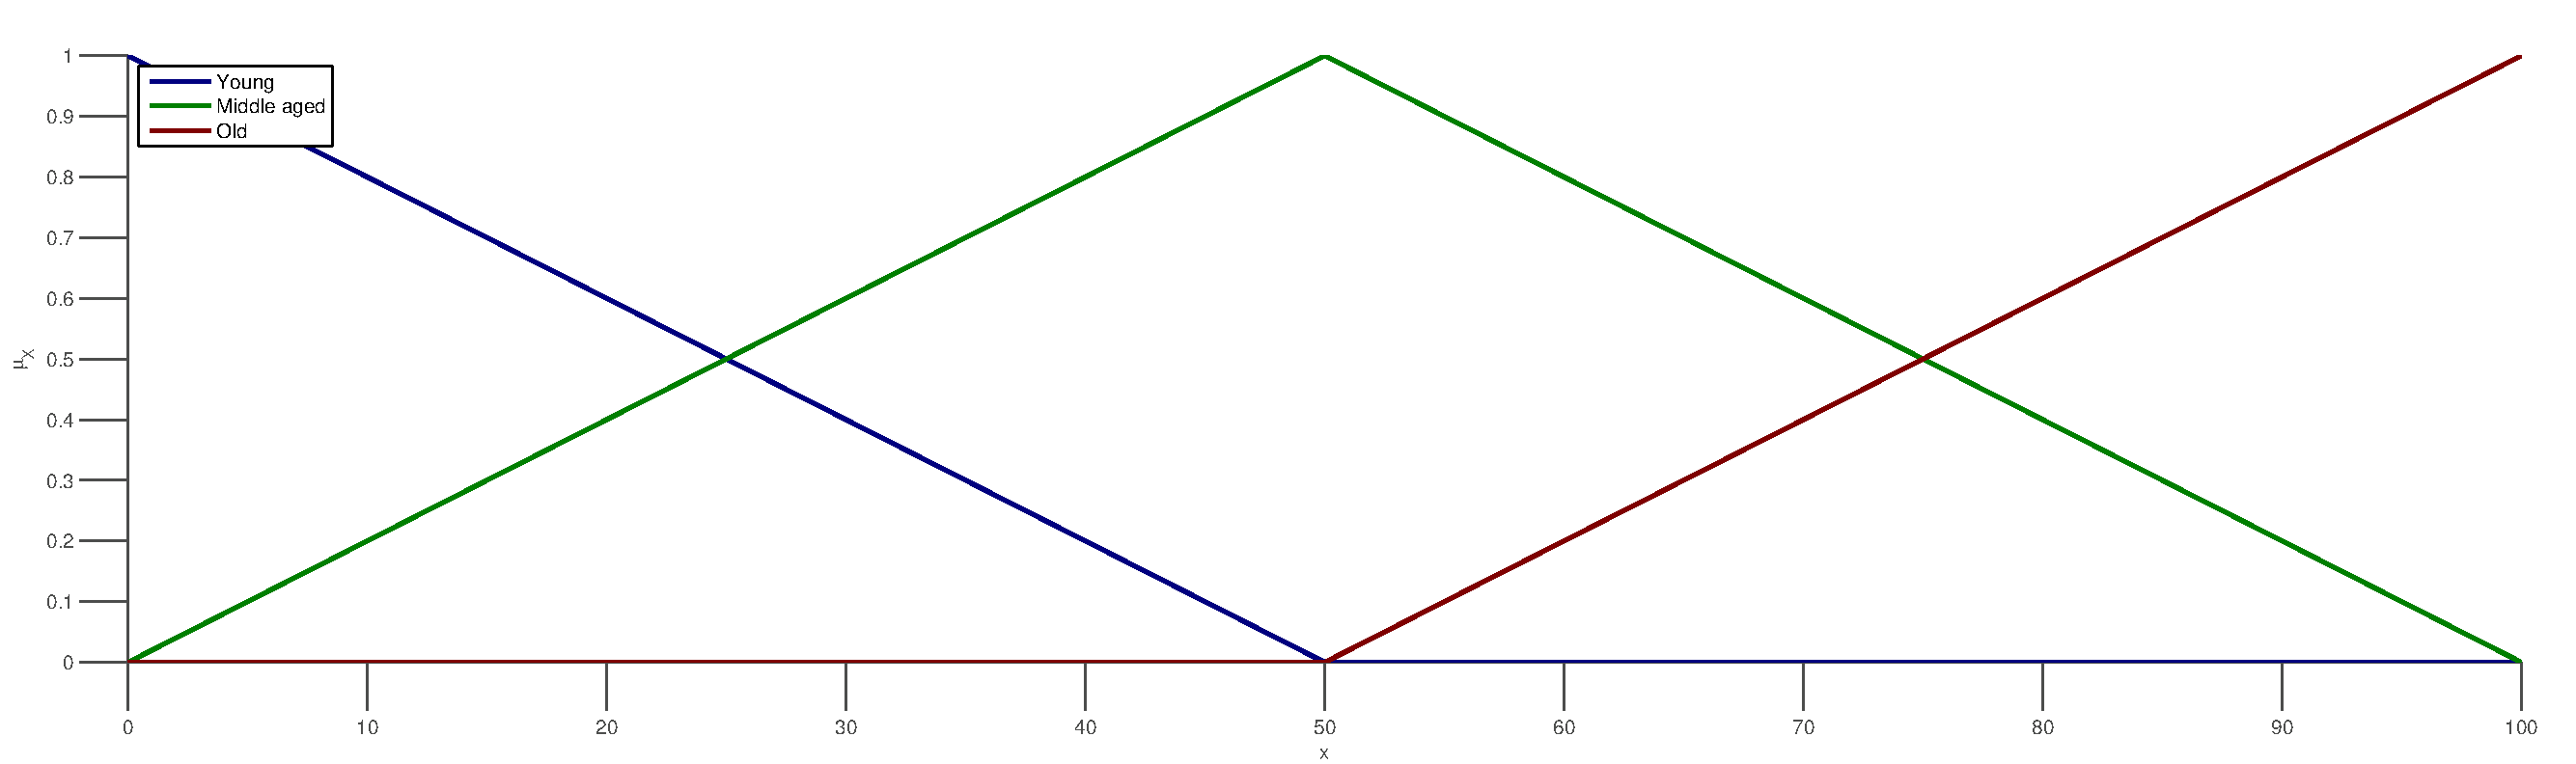
\includegraphics[width=\textwidth]{FMF_ex2}
    \caption[Graphical representation of multiple FMFs]{Fuzzy membership function for $\protect\fuzzyset{A}=\{\text{'Is young'}\}, \protect\fuzzyset{B}=\{\text{'Is middle-aged'\}}\text{ and }\protect\fuzzyset{C}=\{\text{'Is old'}\}$}
    \label{fig:FMF_ex2}
\end{figure}
%------------------------------------------------------------------------------------
\section{Fuzzy logic}
\label{section:fuzzy_logic}
Fuzzy sets and set theory can, in the same manner as classical boolean sets, be used to define logical expressions. Fuzzy logic allows for half-truths, i.e. truth values in the interval [0,1]. Whereas boolean logic is restricted to truth values of one and zero. The truth value T of a fuzzy preposition P is, therefore a mapping from [0,1] to the universe T, as can be seen in \ref{eq:fuzzy-logic-mapping} \cite{ross2009fuzzy}.
\begin{equation}
    T:u\in U\rightarrow (0,1)
    \label{eq:fuzzy-logic-mapping}
\end{equation}
The truth value of proposition P is therefore given by the membership grade $\mu_{\fuzzyset{A}}(x)$ of $x$ in $\fuzzyset{A}$

Many of the same operators and connectives used in classical logic, does also apply to fuzzy logic. This thesis will only present the rules necessary for the scope of the thesis, which are the following \cite{ross2009fuzzy}:\\
\noindent Negation
\begin{equation}
    T(\fuzzyset{\overline{P}})=1-T(\fuzzyset{P})) {}\label{eq:negation}
\end{equation}
Disjunction
\begin{equation}
    \fuzzyset{P}\lor \fuzzyset{Q}:x \text{ is } \fuzzyset{A} \text{ or } \fuzzyset{B}\quad T(\fuzzyset{P} \lor \fuzzyset{Q})=max(T(\fuzzyset{P}),T(\fuzzyset{Q}))\label{eq:disjunction}
\end{equation}
Conjunction
\begin{equation}
    \fuzzyset{P}\land \fuzzyset{Q}:x \text{ is } \fuzzyset{A} \text{ and } \fuzzyset{B}\quad T(\fuzzyset{P} \land \fuzzyset{Q})=min(T(\fuzzyset{P}),T(\fuzzyset{Q}))\label{eq:conjunction}
\end{equation}
Implication
\begin{equation}
    \fuzzyset{P}\to \fuzzyset{Q}: x \text{ is } \fuzzyset{A} \text{, then }x \text{ is } \fuzzyset{B}
    \label{eq:implication}
\end{equation}
\[ T(\fuzzyset{P}\to \fuzzyset{Q})=T(\fuzzyset{\overline{P}}\lor\fuzzyset{Q})=max(T(\fuzzyset{\overline{P}}),T(\fuzzyset{Q}))  \]


\noindent Implication can also be written in rule based form
\[ \fuzzyset{P} \to \fuzzyset{Q} \text{ is,  IF } x \text{ is } \fuzzyset{A} \text{ , THEN } t \text{ is } \fuzzyset{B}\]
\[ \Leftrightarrow \]
\[  R=(\fuzzyset{A}\times\fuzzyset{B})\cup (\overline{\fuzzyset{A}}\times \fuzzyset{Y})\]
\noindent With the membership function:
\begin{equation}
    \mu_{\fuzzyset{R}}(x,y)=max[\mu_{\fuzzyset{A}}(x)\land\mu_{\fuzzyset{B}}(y),(1-\mu_{\fuzzyset{A}}(x))]
    \label{eq:implication-orig}
\end{equation}
Equation \ref{eq:implication-orig} is the fuzzy equivalent to the material implication  $\neg A \lor B$ used in traditional boolean logic\cite{ying2002implication}, where $\neg A = 1-\mu_{\fuzzyset{A}}(x)  $ and $B = \mu_{\fuzzyset{A}}(x)\land\mu_{\fuzzyset{B}}(y)$. However, fuzzy logic has multiple implication operators \cite{ross2009fuzzy}. The work in this thesis will use Mamdani's implication, see equation \ref{eq:mamdani}, since it is the most commonly used one.
\begin{equation}
    \mu_{\fuzzyset{R}}(x,y)=min[\mu_{\fuzzyset{A}}(x),\mu_{\fuzzyset{B}}(x))]
    \label{eq:mamdani}
\end{equation}




%------------------------------------------------------------------------------------
\section{Fuzzy (rule-based) systems}
Fuzzy logic can be used to model complex systems described in natural language, originally written to be interpreted by humans. Such knowledge can often be written as rules in the following form \cite{ross2009fuzzy}.
\begin{equation}
    \text{IF premise (antecedent), THEN conclusion (consequent)}
\end{equation}
Combining multiple rules enables one to describe complex systems in a relatively simple structure. Rules can, furthermore, contain multiple antecedents and consequents. However, this raises the question of how multiple antecedents, as shown in rule \ref{eq:conj-ant}, can be  decomposed into a single antecedent and the rules aggregated into a single consequent \cite{ross2009fuzzy}.
\begin{equation}
    \text {IF $x$ is $\fuzzyset{A_1}$ and $\fuzzyset{A_2}$ \dots and $\fuzzyset{A_L}$ THEN $y$ is $\fuzzyset{B_s}$}
    \label{eq:conj-ant}
\end{equation}
Conjunctive antecedents can be rewritten as a new fuzzy set

\[ \fuzzyset{A_s}=\fuzzyset{A_1}\cap \fuzzyset{A_2} \cap \dots \cap \fuzzyset{A_L} \]
with the membership function
\[ \mu_{\fuzzyset{A_S}}(x)=min \left [\mu_{\fuzzyset{A_1}}(x),\mu_{\fuzzyset{A_2}}(x),\dots,\mu_{\fuzzyset{A_3}}(x) \right ] \]
Rule \ref{eq:conj-ant} can then be rewritten as
\[ \text{IF $\fuzzyset{A_S}$ THEN $\fuzzyset{B_S}$} \]
Disjunctive antecedents can similarly be written as
\[ \fuzzyset{A_s}=\fuzzyset{A_1}\cup \fuzzyset{A_2} \cup \dots \cup \fuzzyset{A_L} \]
\[ \mu_{\fuzzyset{A_S}}(x)=max \left [\mu_{\fuzzyset{A_1}}(x),\mu_{\fuzzyset{A_2}}(x),\dots,\mu_{\fuzzyset{A_3}}(x) \right ] \]
The same principle can be applied to find the overall consequent when multiple rules apply. Conjunctive rules where both consequents must be applied can be found by  the fuzzy intersection of all the rule consequents. Whereas disjunctive rules use the fuzzy union of the rule consequents.



\section{A fuzzy logic model for COLREGs}
\label{section:model}
\todo{Move section to Impl?}
Antecedents consequents and rules are needed in order to make a fuzzy system for a COLREGs compliant auto pilot. The model used in this thesis is created by \textcite{perera2012intelligent} and has four antecedents, two consequents and an extensive rule set of nearly 200 rules. The antecedents used are: relative bearing to the target vessel, relative course of the target vessel, distance between the vessels, and the ratio between the vessels speed. The main vessels relative bearings are divided into ten sets. These resulting sectors represent the different sets in the relative course universe [0, 360]. The relative courses of the target vessel are ,likewise, divided into eight sectors, which represent sets in the relative course universe [0, 360]. The distance universe consist of three sets, representing radii from the main vessel, called $R_A, R_B$ and $R_{VD}$. $R_{VD}$ is the vessel domain into which other vessel shall not enter. $R_A$ and $R_B $depicts the area around the main vessel in which other vessels are detected. $R_A$ when the main vessel is the give way vessel and $R_B$ when it is the stand on vessel. A graphical representation of the bearing, range and course sectors can be seen in figure \ref{fig:model}. The final antecedent, $\text{speed ratio} =\frac{V_{target}}{V{main}}$, consist of three sets: $<1, \approx1 \text{ and } >1$.
Visualizations of the antecedent FMFs, as well as their distribution in their corresponding universes, can be seen in figure \ref{fig:antecedent_fmfs}.

Finally a rules set is needed to connect the antecedents with the consequents. The rule set used for this thesis is based on  the rules, seen in table \ref{tab:rules} developed by \textcite{perera2012intelligent}. A few rules have furthermore been added to handle overtake scenarios. These can be seen in table \ref{tab:rules_own}
\todo{Explain tables?}

An analysis and optimization of the values used to specify the FMFs and the rules in the rule set are unfortunately outside of the scope for this thesis. The values are therefore used as specified in previous research \cite{perera2012intelligent}, with the exception of a few added rules to ensure collisions avoidance when one vessel is overtaking another.


\begin{figure}[H]
    \centering
    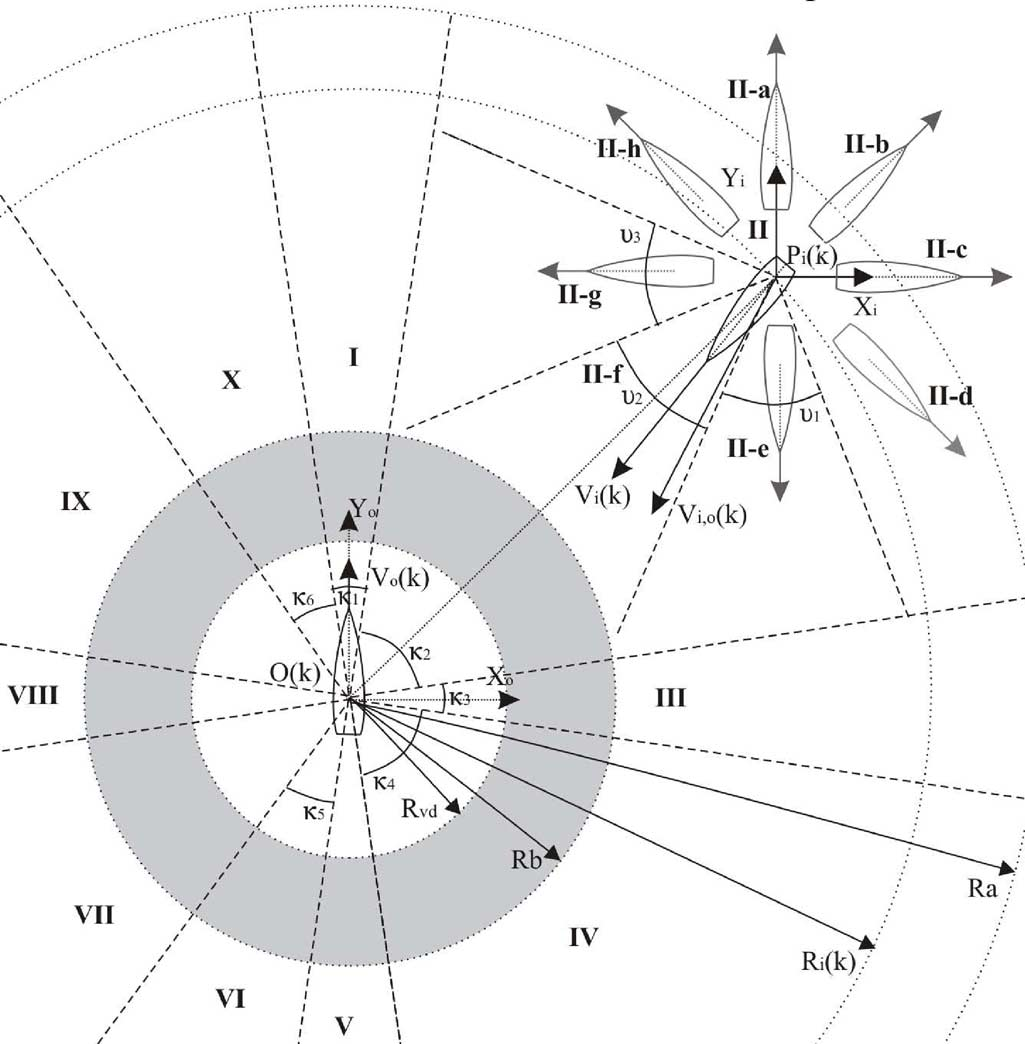
\includegraphics[width=\linewidth]{Figures/model}
    \caption{Mathematical representation of the inputs to a FIS for a two vessel collision situation\cite{perera2012intelligent}}
    \label{fig:model}
\end{figure}

\begin{figure}[H]
    \begin{tabular}{cc}

        \subfloat[Relative bearing of the target vessel from the main vessel]{
            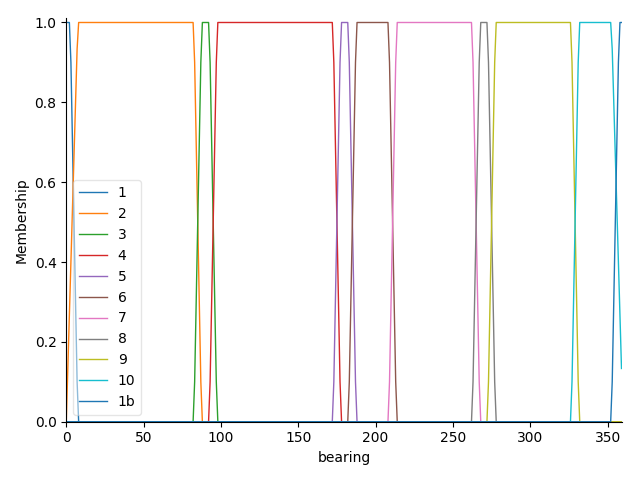
\includegraphics[width=.49\linewidth]{Figures/FMF_bearing}
        } &
        \subfloat[Relative course of the target vessel to the main vessel]{
            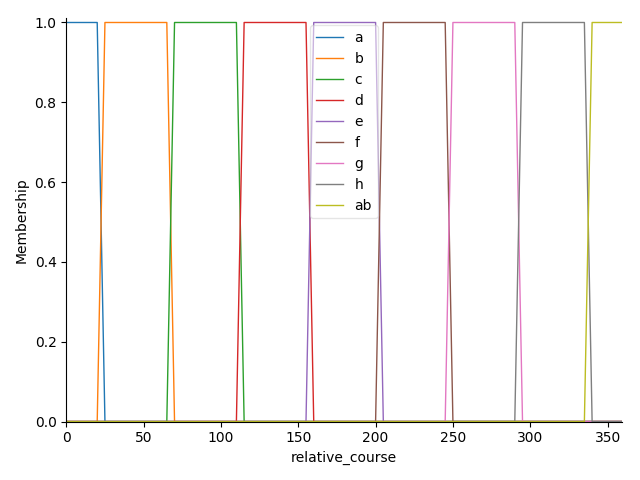
\includegraphics[width=.49\linewidth]{Figures/FMF_rel_course}
        }   \\
        \subfloat[Speed ratio target vessel/main vessel]{
            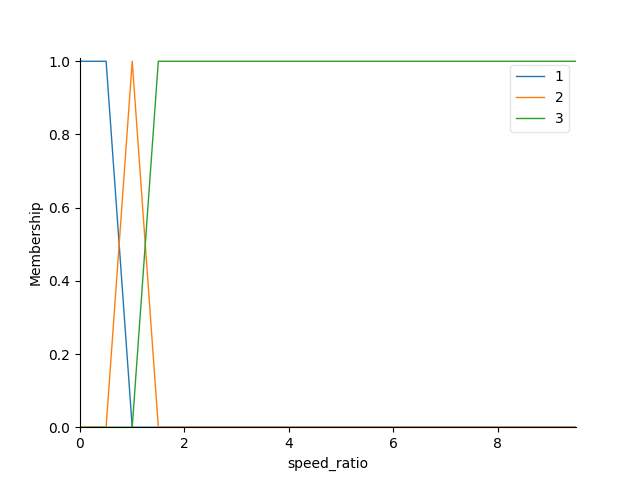
\includegraphics[width=.49\linewidth]{Figures/FMF_speed_ratio}
        } &
        \subfloat[Distance between the main vessel and the target vessel]{
            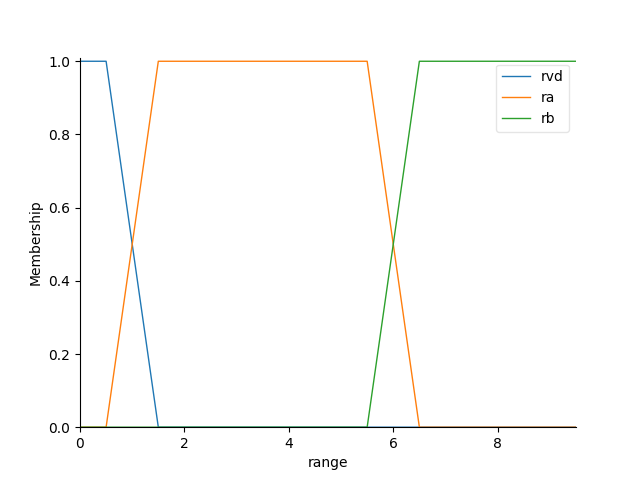
\includegraphics[width=.49\linewidth]{Figures/FMF_range}
        }
    \end{tabular}

    \caption{Antecedent FMFs}
    \label{fig:antecedent_fmfs}
\end{figure}



\begin{figure}[H]

    \begin{tabular}{cc}

        \subfloat[Course change of the main vessel]{
            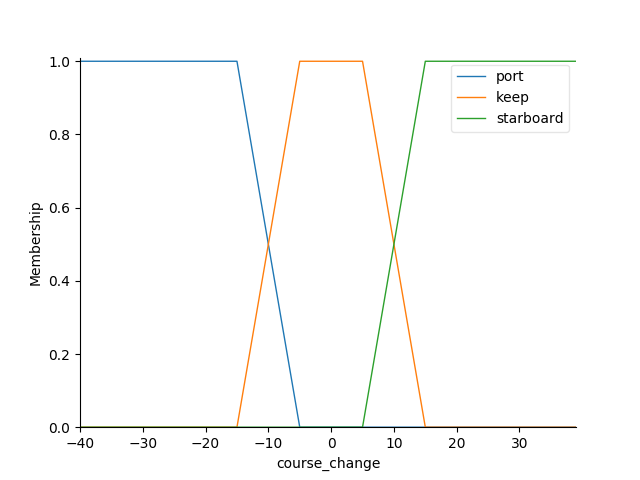
\includegraphics[width=.45\linewidth]{Figures/FMF_course_change}
        } &
        \subfloat[Speed change of the main vessel]{
            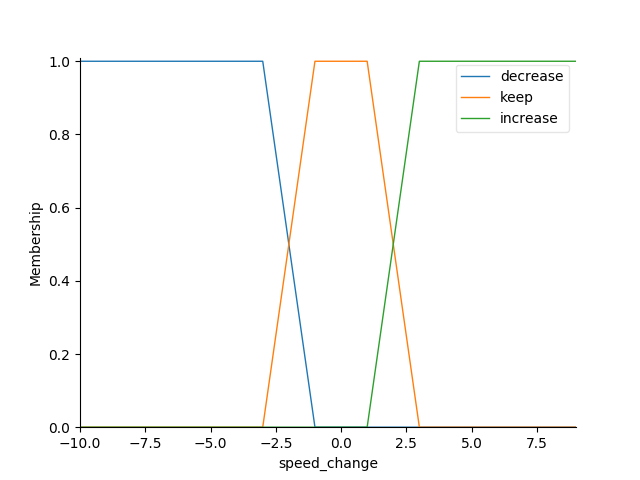
\includegraphics[width=.45\linewidth]{Figures/FMF_speed_change}
        }
    \end{tabular}
    \caption{Consequent FMFs}
    \label{fig:consequent_fmfs}
\end{figure}





\section{Mamdani's fuzzy inference method}
\label{section:FIS}
This thesis will, as mentioned in section \ref{section:fuzzy_logic}, use the Mamdani implication operator in its Fuzzy Inference System (FIS). Mamdani's method was chosen since it is the most common one in practice literature \cite{ross2009fuzzy}.


The following subsections will explain Mamdani's method by going through an example based on the model presented in section \ref{section:model}. The example uses a scenario where two vessels are located in a 2 dimensional 10*10 NM Cartesian coordinate system.\\
Vessel A starts at coordinate (0; -4,5) with heading 0, speed 5 kts and rate of turn 2 degrees per second.\\
Vessel A starts at coordinate (-4,5; -4,5) with heading 203, speed 10 kts and rate of turn 2 degrees per second.
The initial state of the scenario is depicted in figure \ref{fig:scenario_1a}
\begin{figure}[H]
    \centering
    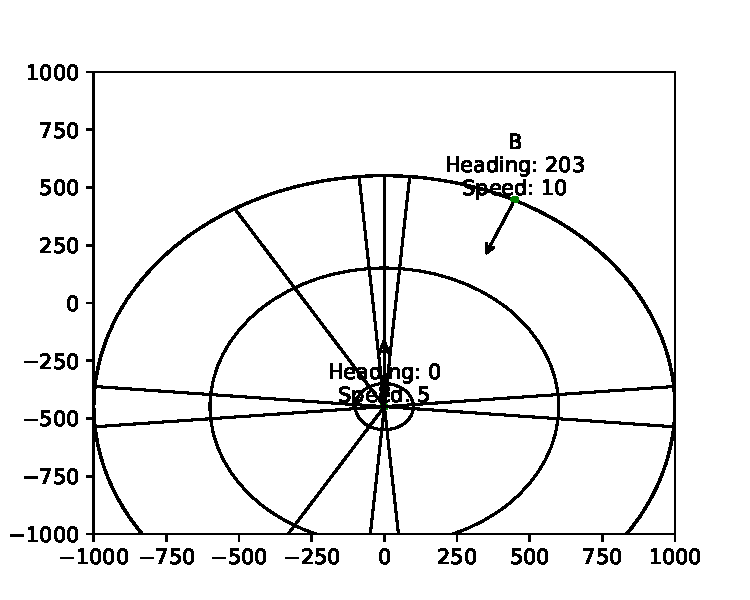
\includegraphics[width=\textwidth]{Figures/scenario_1a}
    \caption{Initial state of the example scenario}
    \label{fig:scenario_1a}
\end{figure}


A FIS can be said to consist of six steps \cite{fis_princeston}:
\begin{enumerate}
    \item Rule determination
    \item Input fuzzification
    \item Combination of antecedents
    \item Obtain consequences
    \item Aggregate consequences
    \item Defuzzification
\end{enumerate}

This example will use a subset of the rules used in the real system.
The rules used are:
\begin{enumerate}[label=\textbf{Rule \arabic*},ref=Rule \arabic*]
    \item \label{rule:1} IF target in sector II AND relative course is in sector f  AND speed ratio is greater than 1  AND range is $R_vd$ OR $R_b$ OR $R_a$ \\THEN change course to starboard  AND  reduce speed.
    \item IF target in sector II AND relative course is in sector e AND  speed ratio is greater than 1  AND  range is $R_vd$ OR $R_b$ OR $R_a$ \\THEN change course to starboard  AND  reduce speed.
\end{enumerate}

Next the crisp values, gained when applying the model presented in section \ref{section:model} on the scenario in figure \ref{fig:scenario_1a}, are fuzzified. The target vessel is located in sector II with a relative bearing of 26,7\textdegree, which results in a membership value of 1 in sector 2 as shown by the red line in figure \ref{fig:FMF_bearing_fuzzified}

The same principle is applied to the three other inputs: relativist course, distance, and speed ratio. Distance and speed ratio will also, in this case, yield membership values of 1, for the fuzzy sets distance $R_a$ and speed ratio>1 . However, the relative course of 203 is located in the fuzzy area between sector 2-e and 2-f which results in membership values of 0,4 and 0,6 respectively, as shown in figure \ref{fig:FMF_rel_course_fuzzified}.
\begin{figure}[H]

    \begin{tabular}{cc}

        \subfloat[Bearing antecedent]{
            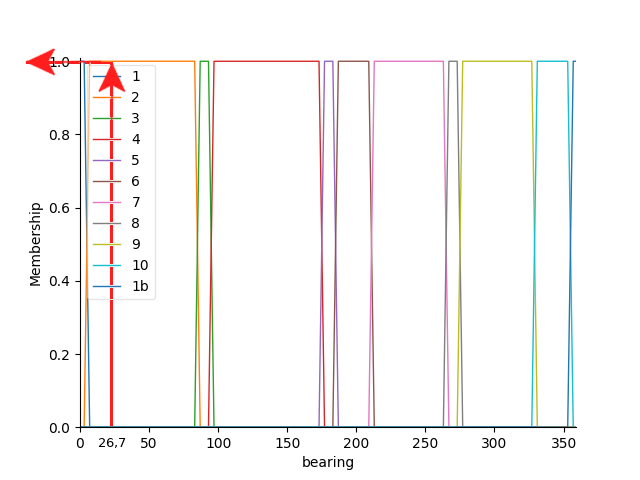
\includegraphics[width=.45\linewidth]{Figures/FMF_bearing_fuzzified}
            \label{fig:FMF_bearing_fuzzified}
        } &
        \subfloat[Relative course antecedent]{
            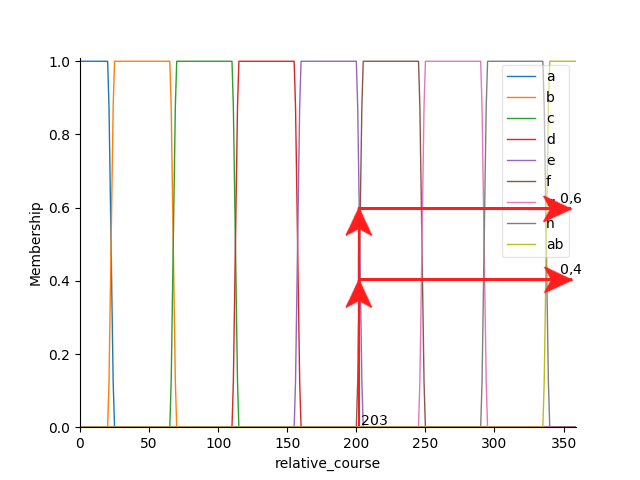
\includegraphics[width=.45\linewidth]{Figures/FMF_rel_course_fuzzified}
            \label{fig:FMF_rel_course_fuzzified}
        }
    \end{tabular}
    \caption{Fuzzified antecedent FMFs for the example scenario}
\end{figure}

The membership values gained for the individual antecedents can then be combined using the AND and OR operators specified in the rule set. This results in the following calculations.
\begin{equation}
    Rule 1: min(1; 0,6; 1; max(0;0;1))=0,6
    \label{eq:ant_comb_rule_1}
\end{equation}
\begin{equation}
    Rule 2: min(1; 0,4; 1; max(0;0;1))=0,4
    \label{eq:ant_comb_rule_2}
\end{equation}

Mamdani's inference method is then used on each rule to obtain the consequent value. This is done by taking the minimum of the antecedent value from the previous step and the consequent. The result is a clipped consequent FMF, as seen in figures \ref{fig:ex_cons_1} and \ref{fig:ex_cons_2}


\begin{figure}[H]

    \begin{tabular}{cc}

        \subfloat[Course change of the main vessel]{
            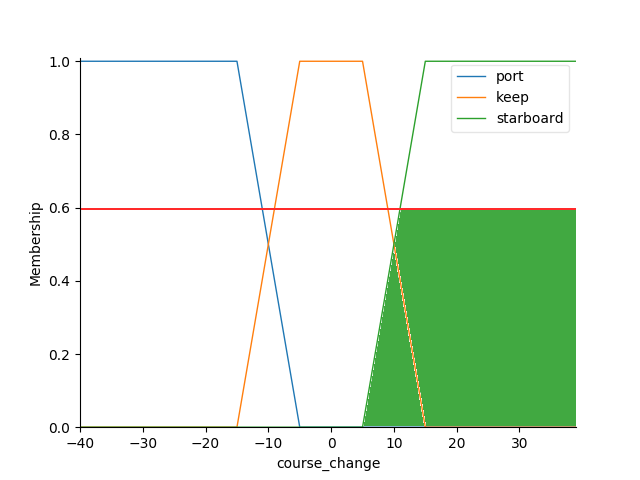
\includegraphics[width=.45\linewidth]{Figures/FMF_course_change_conseq_ex_06}
        } &
        \subfloat[Speed change of the main vessel]{
            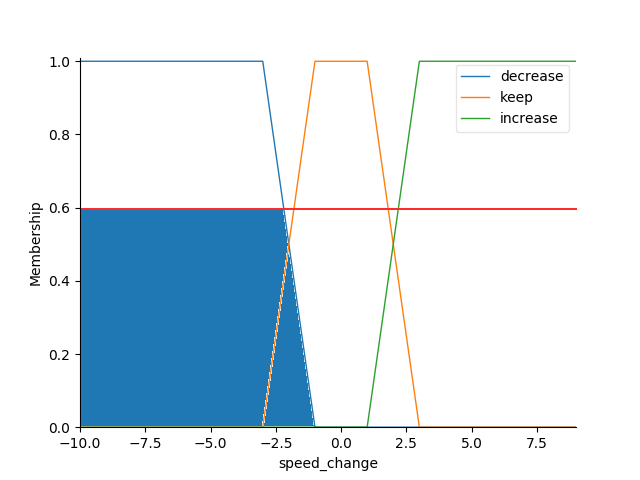
\includegraphics[width=.45\linewidth]{Figures/FMF_speed_change_conseq_ex_06}
        }
    \end{tabular}
    \caption{Consequent FMFs for rule 1 after applying Mamdani's inference method }
    \label{fig:ex_cons_1}
\end{figure}


\begin{figure}[H]

    \begin{tabular}{cc}

        \subfloat[Course change of the main vessel]{
            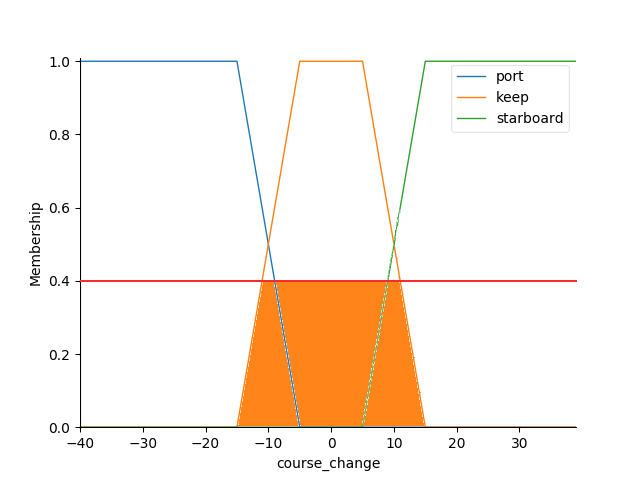
\includegraphics[width=.45\linewidth]{Figures/FMF_course_change_conseq_ex_04}
        } &
        \subfloat[Speed change of the main vessel]{
            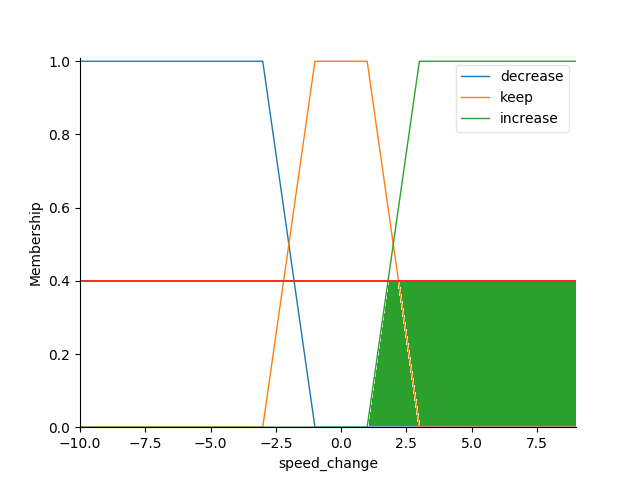
\includegraphics[width=.45\linewidth]{Figures/FMF_speed_change_conseq_ex_04}
        }
    \end{tabular}

    \caption{Consequent FMFs for rule 2 after applying Mamdani's inference method }
    \label{fig:ex_cons_2}
\end{figure}

The clipped consequents, one for each rule, must then be combined. This is achieved by taking the maximum of each consequent, to create a combined FMF. The result is presented in figure \ref{fig:ex_cons_tot}

\begin{figure}[H]

    \begin{tabular}{cc}

        \subfloat[Course change of the main vessel]{
            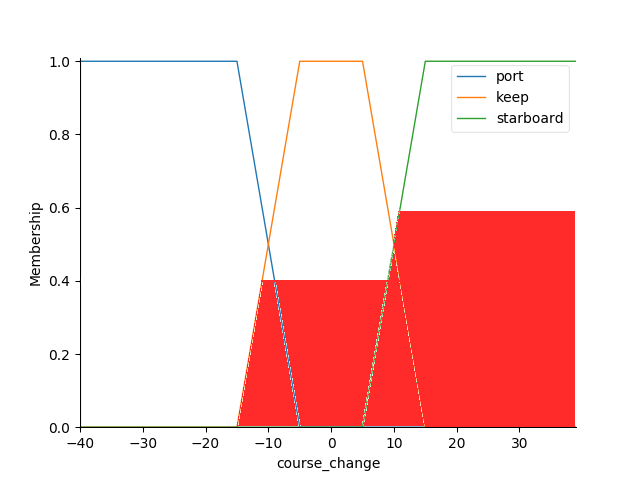
\includegraphics[width=.45\linewidth]{Figures/FMF_course_change_conseq_ex_tot}
        } &
        \subfloat[Speed change of the main vessel]{
            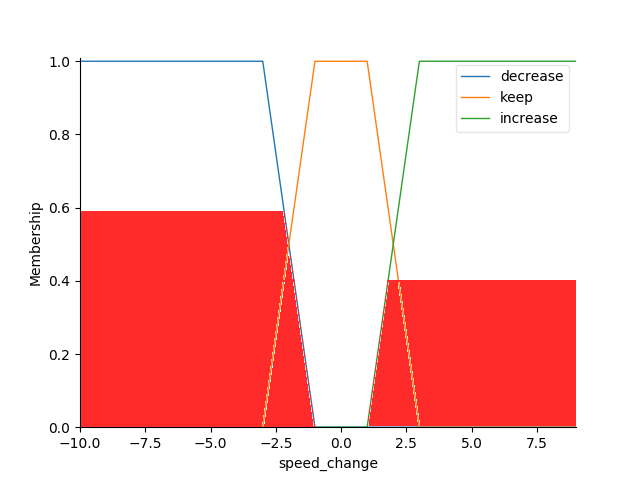
\includegraphics[width=.45\linewidth]{Figures/FMF_speed_change_conseq_ex_tot}
        }
    \end{tabular}

    \caption{Combined Consequent FMFs for the example scenario}
    \label{fig:ex_cons_tot}
\end{figure}

Finally the fuzzy sets gained from the previous step need to be converted into a crisp numerical value that can be used by the auto pilot. This process is called defuzzification and is in this case achieved by calculating the centroid value of FMFs in figure \ref{fig:ex_cons_tot}. The results are a +15.5\textdegree course change and a -1,7 knot speed change.